\section{Model Wind Tunnel Experiments}
\label{MWTE}

\subsection{Scaling Hyper-parameters Invariant LM}
Tensor Program~\citep{yang2022tensor, yang2023tensor} proposes a framework to stabilize the hyper-parameters for models with different scales. The main part of the Tensor Program is the width scaling~\citep{yang2022tensor} and the depth scaling~\citep{yang2023tensor}. The former technique supports CerebrasGPT~\citep{dey2023cerebras} to predict the loss of LLMs more accurately. In MiniCPM, we use both two scaling techniques. The specific scaling operations are listed in Table~\ref{tab:mup}. We do not apply the attention softmax scaling techniques~\citep{yang2022tensor}. Despite ~\cite{yang2023tensor} observing that depth scaling for a network with block depth larger than two is not satisfying, we find the resulting optimal learning rate is stable empirically.

\subsection{Optimal Batch Size}
We follow ~\cite{kaplan2020scaling} to determine the batchsize from expected loss, with a slight modification from their setting (see Appendix~\ref{app:batchsize}). We conduct experiments on 0.009B, 0.03B, and 0.17B models, respectively, toward this goal. Each model size is trained on 6 batch sizes with a global learning rate of $0.01$ and cosine learning rate scheduler. We observe the trend of the optimal batch size with loss on the C4~\citep{2019t5} dataset (red line in the Figure~\ref{fig:optimalbatchsize}).

\begin{figure}[!htbp]
    \centering
    \begin{minipage}{0.66\textwidth}
        \centering
        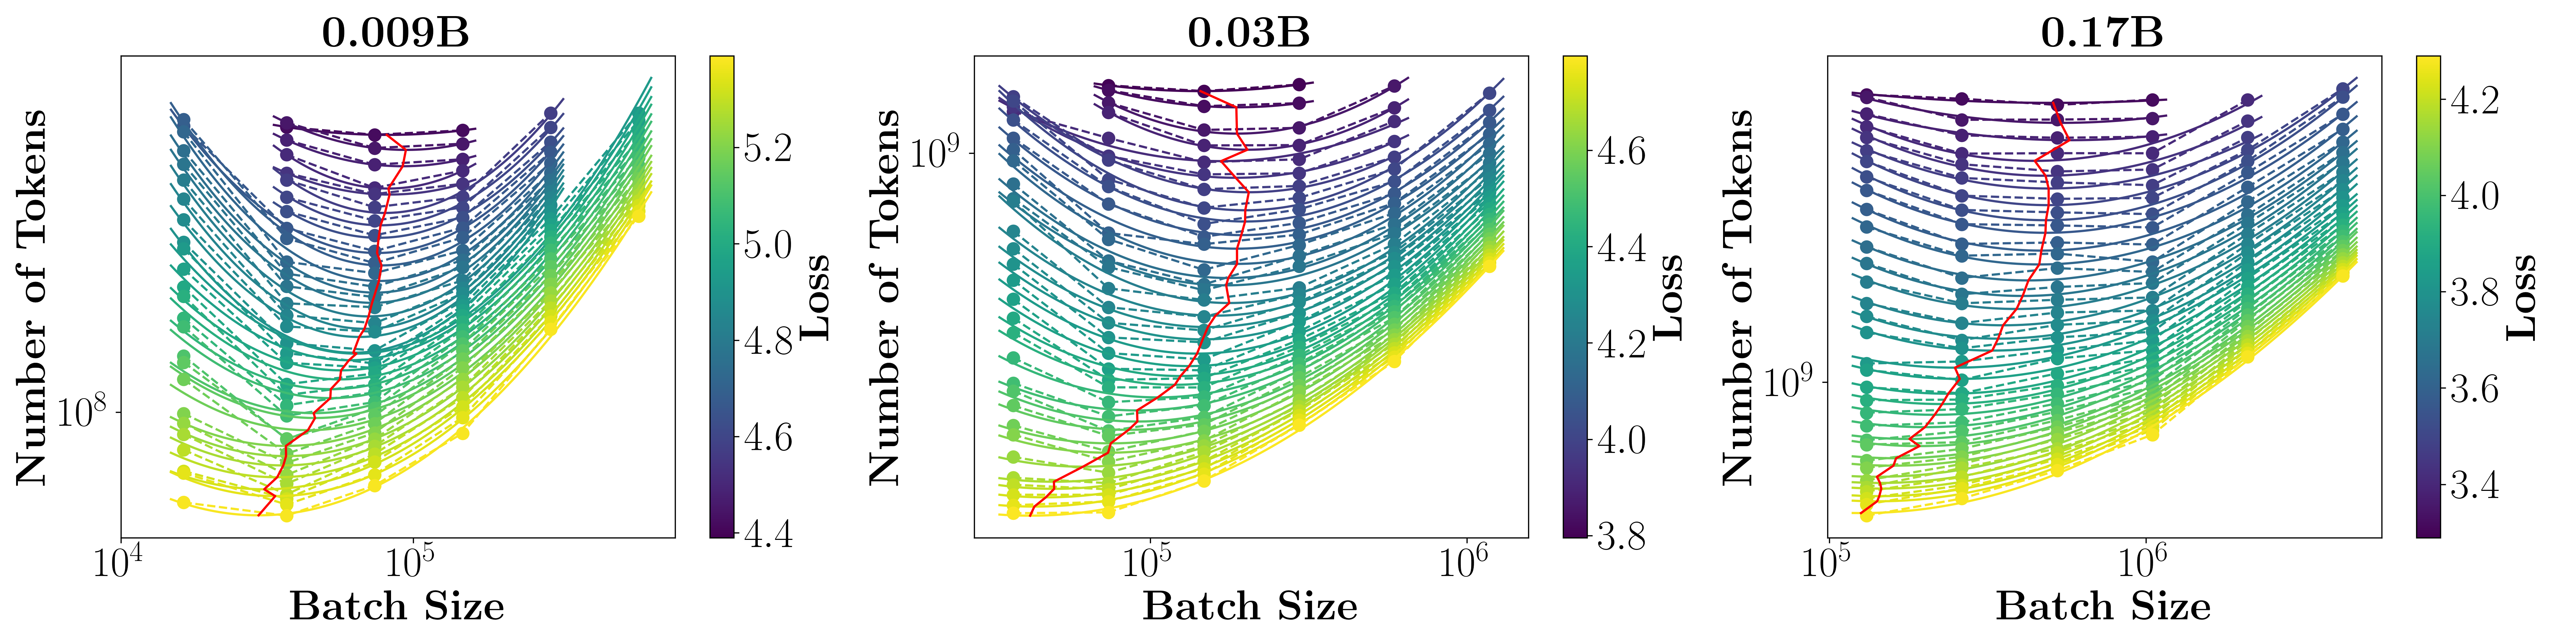
\includegraphics[width=\linewidth]{Fig/batch_size_1.png}
    \caption{We demonstrate the loss curve of three size models trained using different batch sizes. Each vertical line formed by points with a gradient color represents a training curve. Lighter colors denote higher loss.}
    \label{fig:optimalbatchsize}
    \end{minipage}
    \begin{minipage}{0.3\textwidth}
        \centering
        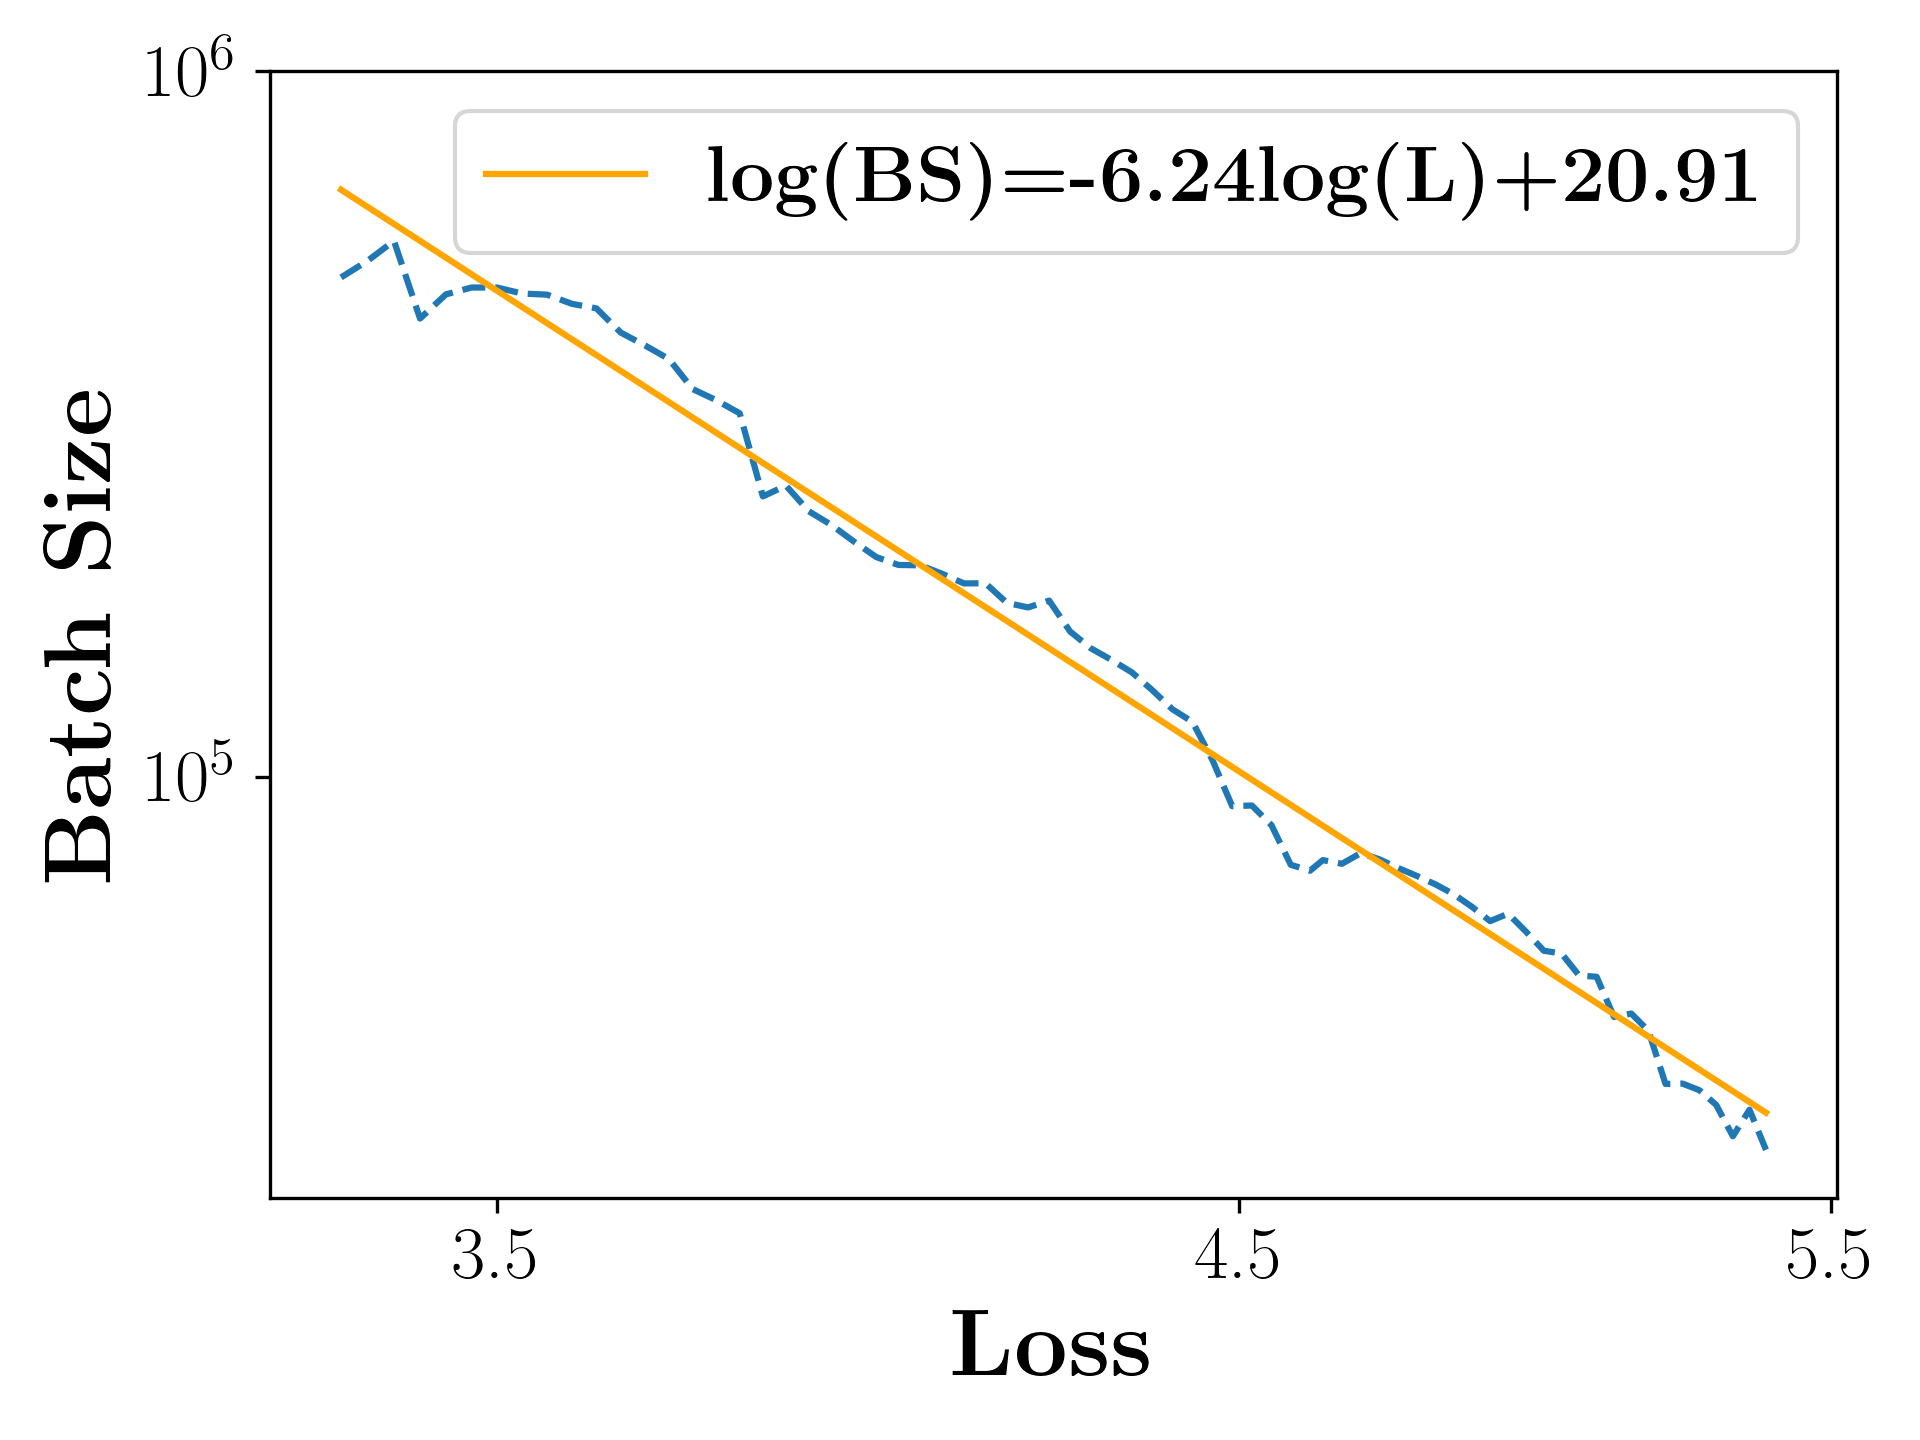
\includegraphics[width=\linewidth]{Fig/batch_size_2.png}
        \caption{The connected optimal batch sizes. }
        \label{fig:optimalbatchsizeconnect}
    \end{minipage}
\end{figure}

As shown in Figure~\ref{fig:optimalbatchsize}, we plot the batch size in the x-axis, and token consumption in the y-axis, the color of the points represents a loss. Thus a horizontal line formed by the color points denotes a training curve. we use parabolas to fit the equal-loss points and connect the minima of the parabolas with red lines. \uline{The lines demonstrate the optimal batch size shifts large as the loss decreases.} We then connect the three lines (see Figure~\ref{fig:optimalbatchsizeconnect}) and find that the lines connect each other well into a linear relationship in the log space, from which we obtain the following relationship between batch size $bs$ and C4 Loss $L$: $ bs = \frac{1.21\times10^9}{L^{6.24}}$. \uline{We note that it might seem strange that the batch size should be estimated from a rough loss prediction that we can only have after training.}

\subsection{Optimal Learning Rate}
\uline{Due to our use of Tensor Program}~\citep{yang2022tensor, yang2023tensor}, \uline{we anticipate that the learning rate, will not undergo significant changes during model scaling.} In Figure~\ref{fig:loss_vs_lr}, we find that although the model size has increased by ten times, the optimal base learning rate~\footnote{The actual learning rate of 2-D tensors will be scaled according to Tensor Program.} does not show a noticeable shift and remains around 0.01.

\vspace{-3mm}
\begin{figure}[htbp]
    \centering
    \begin{minipage}{0.46\linewidth}
        \centering
        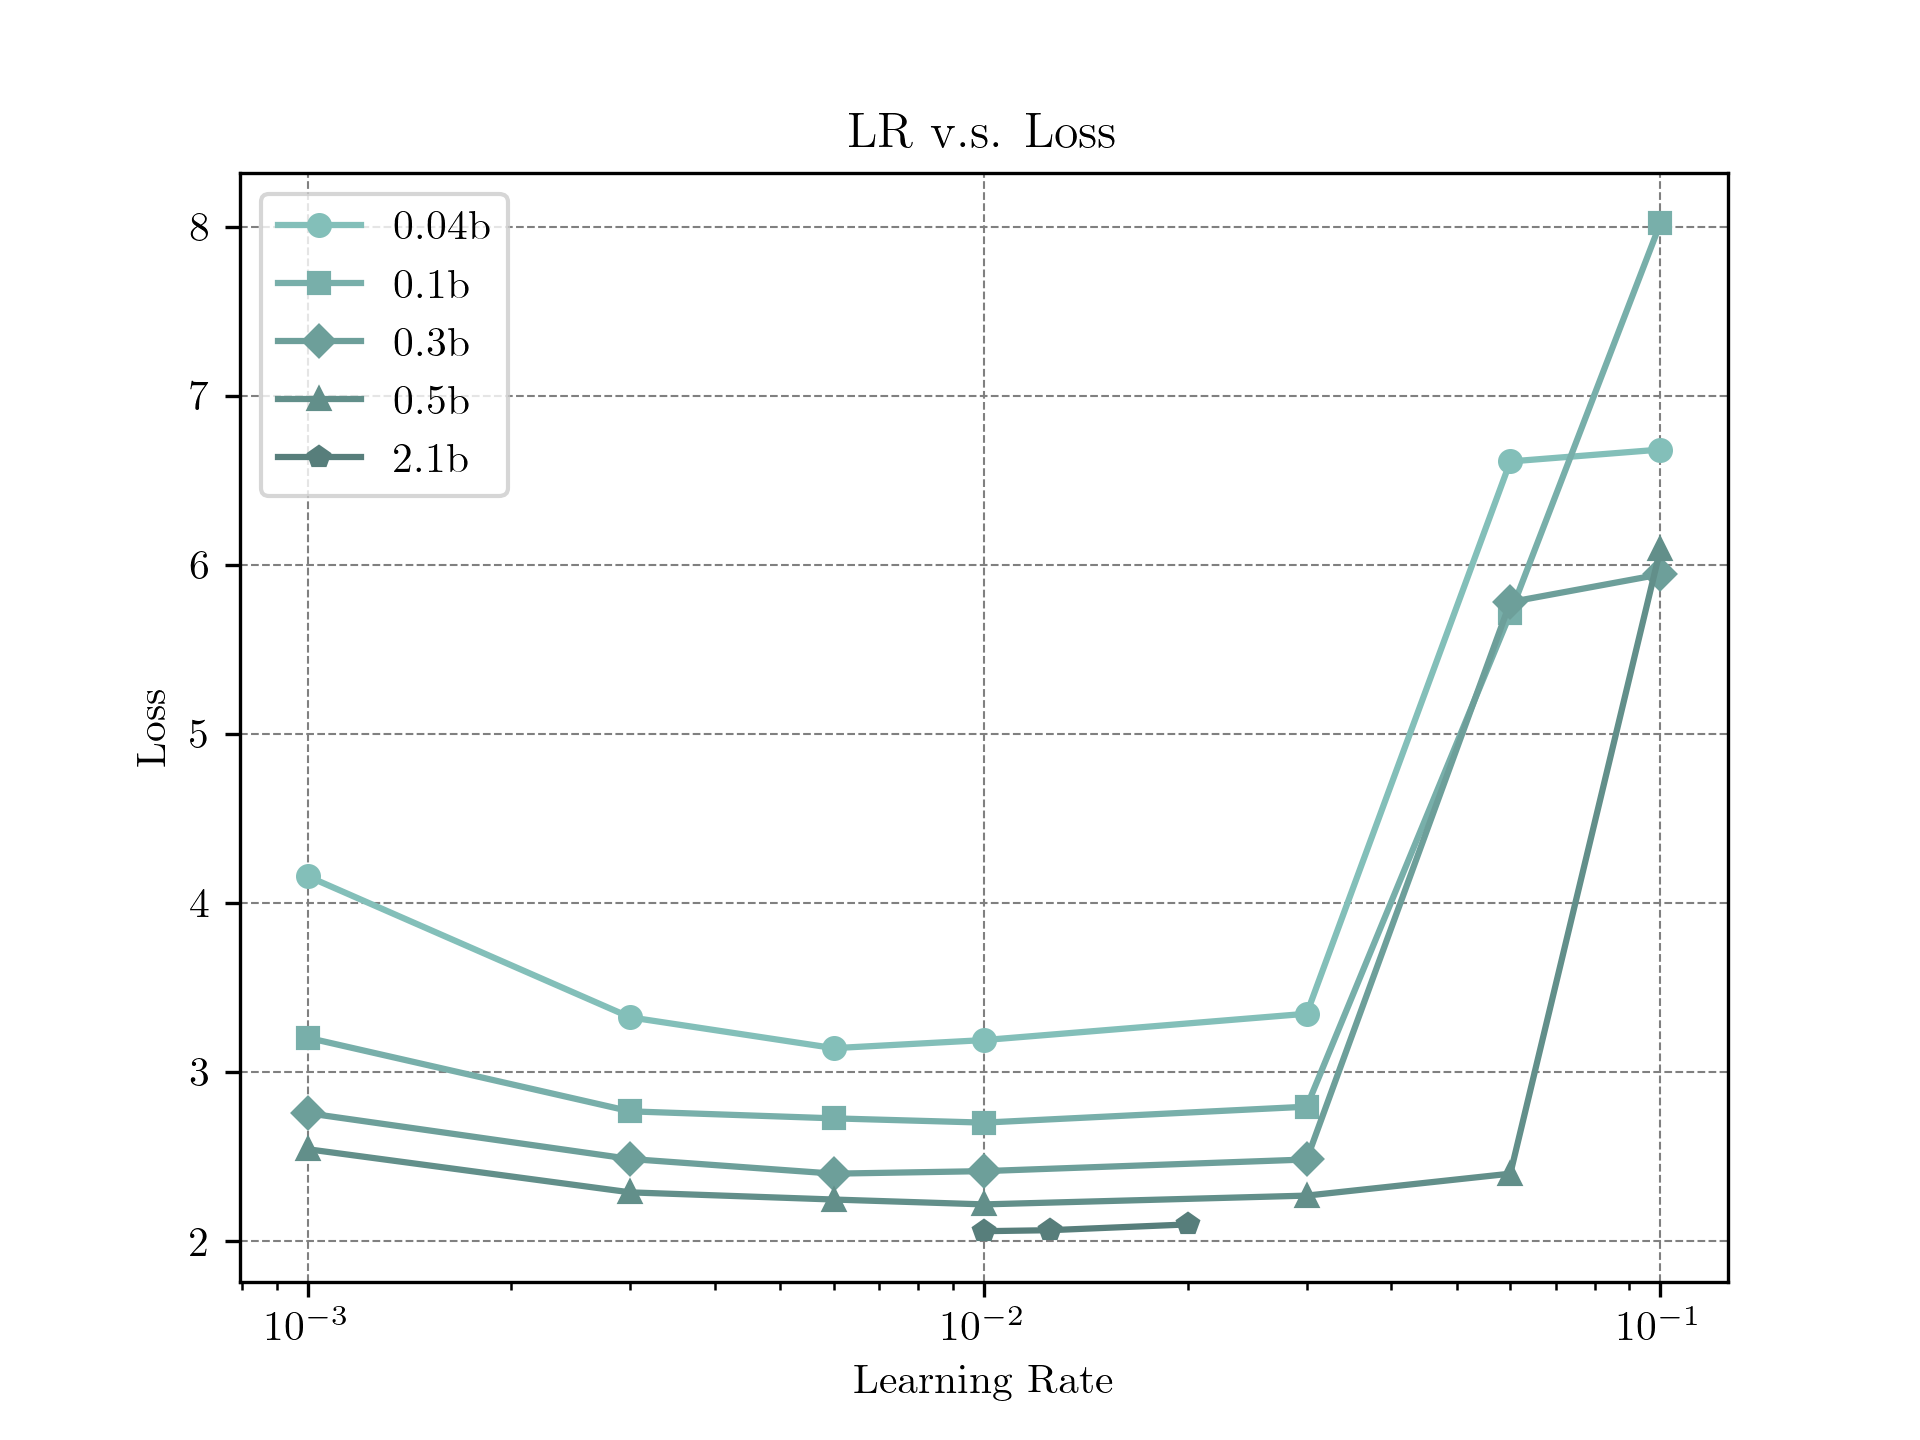
\includegraphics[width=0.9\linewidth]{Fig/loss_vs_lr.png}
        \caption{Loss vs Learning Rate. After applying for the Tensor Program, the learning rate shift becomes minimal.}
        \label{fig:loss_vs_lr}
    \end{minipage}
    \hfill % This adds a little space between the two figures
    \begin{minipage}{0.46\linewidth}
        \centering
        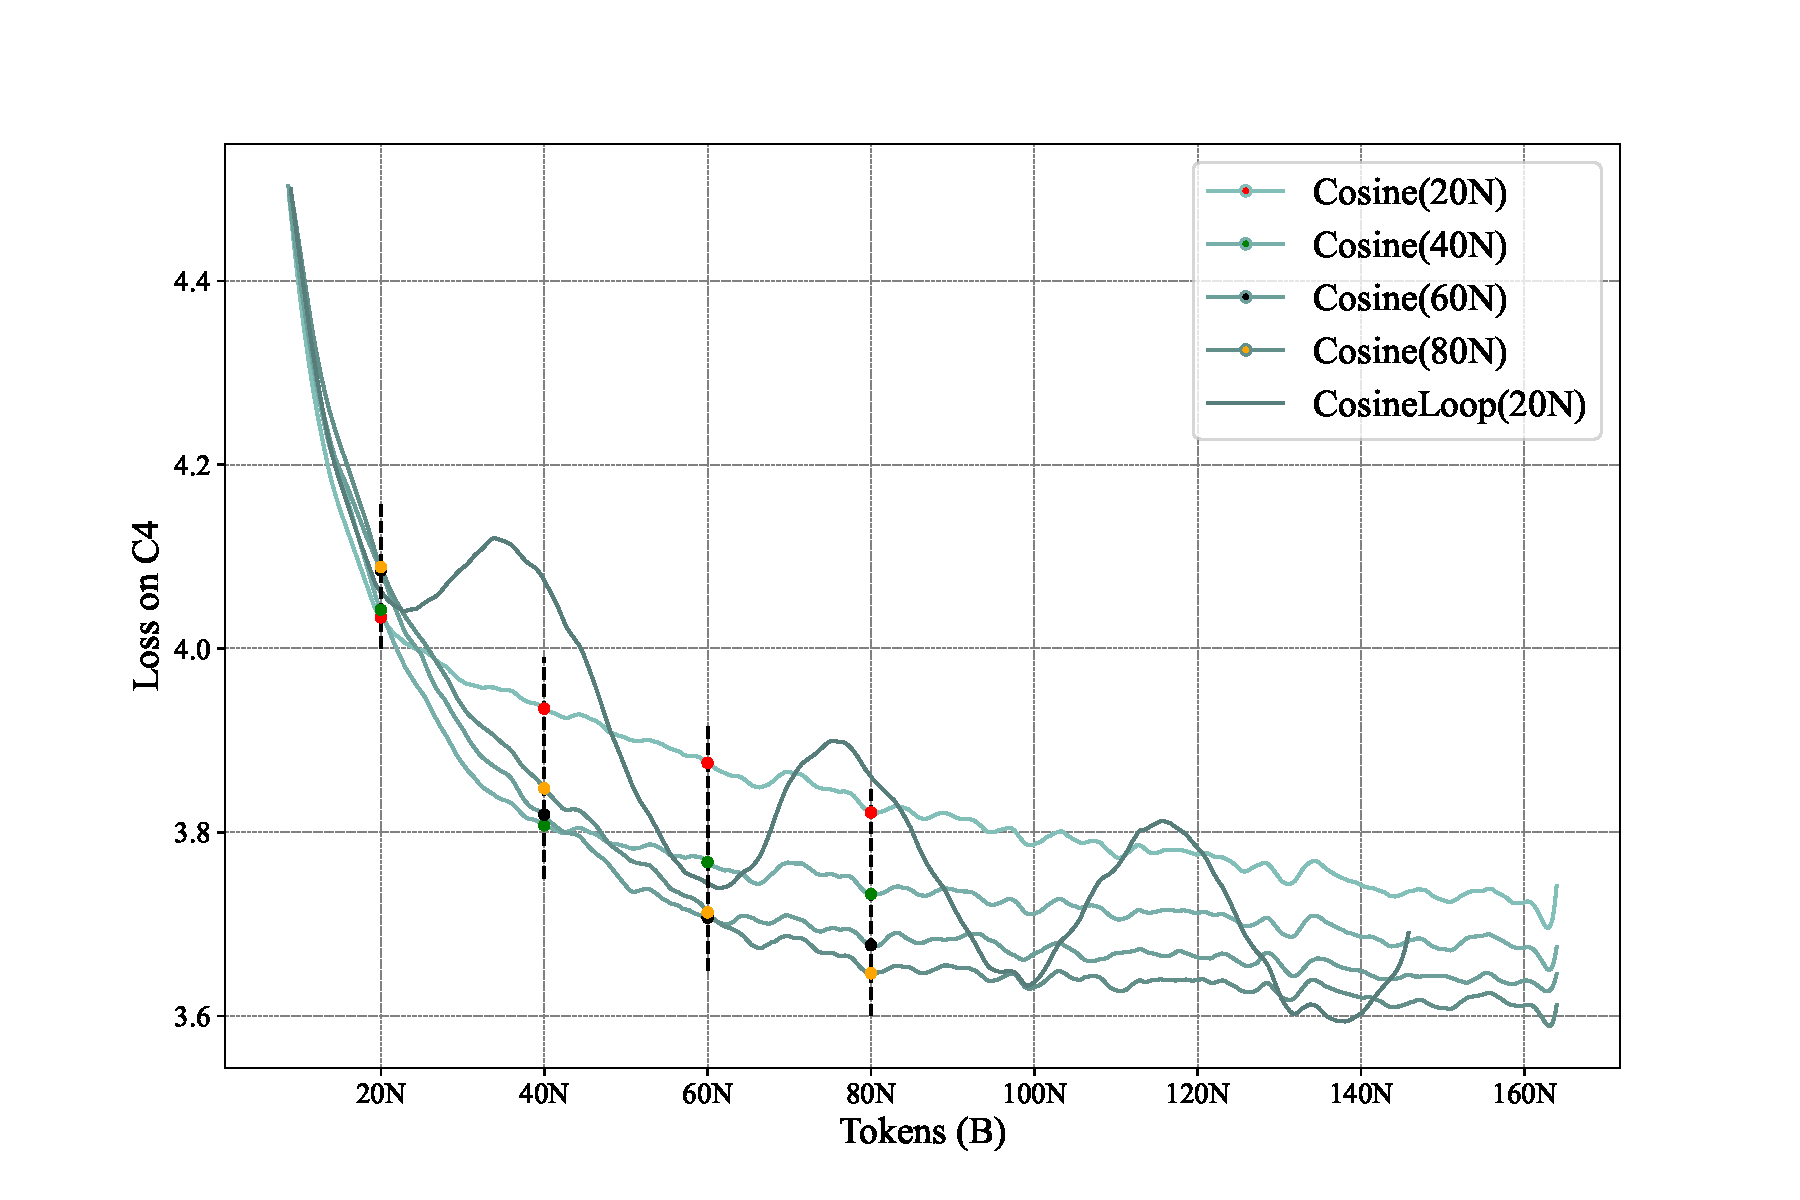
\includegraphics[width=1.0\linewidth]{Fig/cosine_2024-03-26_15-36-16.pdf}
        \caption{Cosine Learning Rate Scheduler with different periods. The Y-axis is the loss on the C4 corpus.}
        \label{fig:cosine_lr}
        \vspace{0.47cm}
    \end{minipage}
\end{figure}
\vspace{-5mm}